\chapter{模型方程:一维双曲守恒律方程}


对于一维双曲守恒律问题的数值求解目标是设计高精度高分辨率的数值格式:
\begin{itemize}
    \item 数值解希望收敛到熵解,至少是弱解;
    \item 在真解相对光滑区域,保持高精度和高计算效率;
    \item 在真解间断的区域,要捕获到间断界面和刻画激波速度,并抑制间断界面附近的数值振荡。
\end{itemize}


\section{数值格式(一)}

直接对守恒律方程(守恒形式或非守恒形式)进行离散,对非线性部分进行冻结系数等近似处理,就可以得到很多格式,例如 Roe 迎风格式,Lax 格式,Lax-Wendroff 格式等。
\begin{example}
    构造迎风格式
    \begin{enumerate}
        \item 基于守恒形式 $u_t + f(u)_x = 0$
              \[
                  v_j^{n+1} =
                  \begin{cases}
                      v_j^n - \frac{\Delta t}{\Delta x}\left(f(v_{j}^n)-f(v_{j-1}^n)\right), & f'(v_j^n) > 0   \\
                      v_j^n - \frac{\Delta t}{\Delta x}\left(f(v_{j+1}^n)-f(v_{j}^n)\right), & f'(v_j^n) \le 0 \\
                  \end{cases}
              \]
        \item 基于非守恒形式 $u_t + a(u) u_x = 0$
              \[
                  v_j^{n+1} =
                  \begin{cases}
                      v_j^n - \frac{\Delta t}{\Delta x} a(v_j^n) \left(v_{j}^n-v_{j-1}^n\right), & a(v_j^n) > 0   \\
                      v_j^n - \frac{\Delta t}{\Delta x} a(v_j^n) \left(v_{j+1}^n-v_{j}^n\right), & a(v_j^n) \le 0 \\
                  \end{cases}
              \]
    \end{enumerate}
\end{example}


\begin{example}
    构造Lax格式
    \begin{enumerate}
        \item 基于守恒形式 $u_t + f(u)_x = 0$
              \[
                  v_j^{n+1} = \frac12 (v_{j-1}^n + v_{j+1}^n)
                  - \frac{\Delta t}{2\Delta x} \left(f(v_{j+1}^n)-f(v_{j-1}^n)\right)
              \]
        \item 基于非守恒形式 $u_t + a(u) u_x = 0$
              \[
                  v_j^{n+1} = \frac12 (v_{j-1}^n + v_{j+1}^n)
                  - \frac{\Delta t}{2\Delta x} a(v_j^n)\left(v_{j+1}^n-v_{j-1}^n\right)
              \]
    \end{enumerate}
\end{example}

\begin{example}
    构造 Lax-Wendroff 格式
    \begin{enumerate}
        \item 基于守恒形式 $u_t + f(u)_x = 0$,记 $A_{j+\frac12}^n = f'(\frac12(v_j^n+v_{j+1}^n))$
              \begin{align*}
                  v_j^{n+1} ={} & v_j^n
                  - \frac{\Delta t}{2\Delta x} \left(f(v_{j+1}^n)-f(v_{j-1}^n)\right)
                  \\ & + \frac{\Delta t^2}{2\Delta x^2}\left\{
                  A_{j+\frac12}^n [f(v_{j+1}^n) - f(v_{j}^n)]
                  - A_{j-\frac12}^n [f(v_{j}^n) - f(v_{j-1}^n)]
                  \right\}
              \end{align*}
        \item 基于非守恒形式 $u_t + a(u) u_x = 0$
              \begin{align*}
                  v_j^{n+1} ={} & v_j^n
                  - \frac{\Delta t}{2\Delta x} a(v_j^n)\left(v_{j+1}^n-v_{j-1}^n\right)
                  \\ & + \frac{\Delta t^2}{2\Delta x^2}\left\{
                  a(v_j^n)^2(v_{j+1}^n - 2 v_j^n + v_{j-1}^n)
                  + \frac12 a(v_j^n)a'(v_j^n)(v_{j+1}^n-v_{j-1}^n)^2
                  \right\}
              \end{align*}
    \end{enumerate}
\end{example}


\begin{example}
    基于守恒形式 $u_t + f(u)_x = 0$,构造 Roe 迎风格式
    \[
        v_j^{n+1} = v_j^n - \frac{\Delta t}{2\Delta x}
        \left\{
        (1+\text{sgn}(a_{j-\frac12}^n))(f(v_{j}^n)-f(v_{j-1}^n))
        + (1-\text{sgn}(a_{j+\frac12}^n))(f(v_{j+1}^n)-f(v_{j}^n))
        \right\}
    \]
    其中 $a_{j+\frac12}^n$ 是 Roe 平均,满足如下等式
    \[
        f(v_{j+1}^n)-f(v_{j}^n) = a_{j+\frac12}^n(v_{j+1}^n-v_j^n)
    \]
\end{example}


\begin{example}[Lax-Friedrichs]
    基于守恒形式 $u_t + f(u)_x = 0$,利用流通分裂技术将其拆分为
    \[
        u_t + f^+(u)_x + f^-(u)_x = 0,\quad f^{\pm}(u) = \frac12(f(u)\pm \alpha u).
    \]
    其中 $\alpha = \max_u |f'(u)|$。对 $f^+$ 和 $f^-$ 分别使用迎风格式可得 Lax-Friedrichs 格式
    \[
        v_j^{n+1} = v_j^n - \frac{\Delta t}{\Delta x}(f^+(v_{j}^n)-f^+(v_{j-1}^n))
        - \frac{\Delta t}{\Delta x}(f^-(v_{j+1}^n)-f^-(v_{j}^n))
    \]
\end{example}

\section{守恒型格式}

对于守恒律方程直接设计的差分格式可能产生错误的结果:得到的数值解可能收敛到不是弱解的某个函数,考虑下面的例子。

\begin{example}
    对于 Burgers 方程 $u_t + u u_x = 0$ 的 Riemann 问题,初值满足
    \[
        u_0(x) =
        \begin{cases}
            0, & x < 0   \\
            1, & x \ge 0
        \end{cases} \quad \Rightarrow \quad  v_j^0 =
        \begin{cases}
            0, & j \ge 0 \\
            1, & j < 0
        \end{cases}
    \]
    使用非守恒形式的迎风格式进行求解
    \[
        v_j^{n+1} = v_j^n - \frac{\Delta t}{\Delta x} v_j^n (v_{j}^n-v_{j-1}^n)
    \]
    单步计算得到的结果为
    \[
        v_j^1 = v_j^0 - \frac{\Delta t}{\Delta x} v_j^0 (v_{j}^0 - v_{j-1}^0)
        =
        \left\{
        \begin{aligned}
             & 0 - 0 = 0,\quad j \ge 0                             \\
             & 1 - \frac{\Delta t}{\Delta x}(1-1) = 1, \quad j < 0
        \end{aligned}
        \right.
    \]
    因此 $v_j^n = v_j^{n-1} = \dots = v_j^1 = v_j^0$,数值格式给出了一个静止不动的解,并且随着网格加密也不会变化。
    这不是满足方程的弱解,因为激波速度 $s = 0$ 不满足 RH 条件。
\end{example}

我们必须将守恒律方程自身所满足的局部守恒性也体现在数值格式中,这自然引出了守恒型格式的概念。

\begin{definition}[守恒型格式]
    称差分格式为守恒型格式,如果它可以表述为如下形式
    \[
        v_{j}^{n+1} = v_j^n - \frac{\Delta t}{\Delta x}\left(
        \hat{f}_{j+\frac12}^n - \hat{f}_{j-\frac12}^n
        \right),\quad \forall\,j
    \]
    其中 $\hat{f}_{j+\frac12} = \hat{f}(v_{j-r},\cdots,v_{j+s})$ 称为数值流通量,满足
    \begin{enumerate}
        \item 连续性:$\hat{f}$ 关于每一个变量都是局部Lipschitz连续的
        \item 相容性:$\hat{f}(v,\dots,v) = f(v)$
    \end{enumerate}
\end{definition}

对守恒型格式关于 $j$ 进行局部地求和并乘以 $\Delta x$,可以得到
\[
    \Delta x\sum_{j=p}^q v_j^{n+1}  = \Delta x\sum_{j=p}^q v_j^n  -  \Delta t
    \left(
    \hat{f}_{q+1/2}^n - \hat{f}_{p-1/2}^n
    \right)
\]
这是离散意义下的局部守恒性,对应的连续意义下的局部守恒性是
\[
    \int_{x_{p-1/2}}^{x_{q+1/2}} u(x,t^{n+1}) \,dx
    =
    \int_{x_{p-1/2}}^{x_{q+1/2}} u(x,t^n)\,dx
    - \int_{t^n}^{t^{n+1}} f(u(x_{q+1/2},t)) - f(u(x_{p-1/2},t))\,dt
\]
给定一个守恒型数值格式,反过来要求给出数值流通量的形式时,也可以利用这个性质,对格式关于 $j$ 进行部分求和,进而推出数值流通量的具体形式。



一般的数值格式可能无法保证得到的解是弱解,守恒型格式由于具有局部守恒性,可以保证得到的一定是弱解,有如下定理:
\begin{theorem}[Lax-Wendroff定理]
    设守恒型差分格式与双曲守恒律相容,当时空网格尺度趋于零时,
    若数值解几乎处处有界并且收敛到某个函数,则极限函数必定是问题的弱解。
\end{theorem}

但是下面的例子表明,守恒型格式不能保证得到的结果是熵解。

\begin{example}
    对于 Burgers 方程 $u_t + u u_x = 0$ 的 Riemann 问题,初值满足
    \[
        u_0(x) =
        \begin{cases}
            -1, & x < 0   \\
            1,  & x \ge 0
        \end{cases} \quad \Rightarrow \quad  v_j^0 =
        \begin{cases}
            -1, & j \ge 0 \\
            1,  & j < 0
        \end{cases}
    \]
    使用守恒形式的 Roe 迎风格式进行求解
    \[
        v_j^{n+1} = v_j^n - \frac{\Delta t}{2\Delta x}
        \left\{
        (1+\text{sgn}(a_{j-\frac12}^n))(f(v_{j}^n)-f(v_{j-1}^n))
        + (1-\text{sgn}(a_{j+\frac12}^n))(f(v_{j+1}^n)-f(v_{j}^n))
        \right\}
    \]
    注意到始终有 $f(v_{j}^0)-f(v_{j-1}^0) = 0$,因此同样有 $v_j^n = v_j^{n-1} = \dots = v_j^1 = v_j^0$,
    数值格式给出了一个静止不动的解,并且随着网格加密也不会变化。
    这是满足方程的弱解,因为激波速度 $s = 0$ 此时满足 RH 条件,但是这不是熵解,因为不满足熵条件 $f'(u_l) \ge s \ge f'(u_r)$。
\end{example}


对于双曲守恒律问题,必须要考虑间断界面的处理,但是守恒型格式仍然可能在间断附近产生数值振荡,
并且守恒型格式只能保证得到弱解而非熵解。为了解决这两个问题,引入了单调格式和TVD格式等概念。

\begin{remark}
    我们默认下文中引入的单调格式、TVD格式等概念都是在守恒型格式前提下的定义,虽然它们的定义中并没有涉及到守恒型格式的要求,
    在某些资料中这些概念的定义可以独立于守恒型格式(例如张强《偏微分方程的有限差分方法》),此时主要讨论的就是守恒型单调格式、守恒型TVD格式等。
    这里默认均为守恒型格式可以简化一些语句的表述。
\end{remark}

\section{单调保持和单调格式}

\begin{definition}
    称方程具有单调保持性质,如果满足:对于单增或单减的初值,任意时刻的熵解均保持相同的单调性。
\end{definition}

\begin{definition}
    称方程具有比较性质,如果满足:
    \[
        u_1(x,0) \le u_2(x,0)\quad(\forall\, x) \quad \Rightarrow \quad
        u_1(x,t) \le u_2(x,t)\quad(\forall\, x,\,\forall\,t > 0)
    \]
\end{definition}

理论分析表明,双曲守恒律问题的熵解具有单调保持性质和比较性质,因此我们也希望设计的数值格式在离散意义下保持相应的性质。

\begin{definition}[单调保持格式]
    称差分格式为单调保持格式,如果满足:对于单增或单减的初值,任意时刻的数值解均具有相同的单调
    性。
\end{definition}

单调保持格式可以避免产生数值振荡,但是单调保持的概念在实践中难以验证。
我们可以加强条件,引入一类要求更强,但实践中更容易验证的概念——单调格式。

\begin{definition}[单调格式]
    称差分格式是单调格式,若它可以表述为如下形式
    \[
        v_j^{n+1} = H(v_{j-r-1}^n,\cdots,v_{j+s}^n),\quad \forall\,j
    \]
    其中 $H$ 关于每一个变量都是非减的,即 $H(\uparrow,\,\cdots,\,\uparrow)$。
\end{definition}


可以证明单调格式是一个更强的概念:

\begin{theorem}
    单调格式一定是单调保持格式,反之未必成立。限于线性格式的范畴,单调格式等价于单调保持格式。
\end{theorem}

\begin{proof}
    取单调的离散值 $v_j^0 \le v_{j+1}^0$,$\forall\, j$,那么
    \[
        v_{j}^1 = H(v_{j-r-1}^0,\cdots,v_{j+s}^0)
        \le H(v_{j-r}^0,\cdots,v_{j+s+1}^0) = v_{j+1}^1
    \]
    归纳可得,对于任意时刻 $t^n$,都有相同的单调性: $v_j^n \le v_{j+1}^n$,$\forall\, j$\,。
    对于线性格式
    \[
        v_j^{n+1} = \sum_{s=-p}^q c_s\, v_{j+s}^n
    \]
    单调保持可以推出所有系数都非负,从而是单调格式。
\end{proof}

如下命题可以用于判断一个三点格式是否是单调格式。
\begin{proposition}
    对于如下形式的三点格式
    \[
        v_{j}^{n+1} = v_j^n - \frac{\Delta t}{\Delta x}\left(
        \hat{f}_{j+\frac12}^n - \hat{f}_{j-\frac12}^n
        \right),\quad \hat{f}_{j+\frac12}=\hat{f}(v_j^n,v_{j+1}^n).
    \]
    显然可以整理为 $v_{j}^{n+1} = H(v_{j-1}^n,v_j^n,v_{j+1}^n)$。
    若数值流通量 $\hat{f}$ 满足如下条件
    \[
        \partial_1\hat{f}(u,v) \ge 0,\quad
        - \partial_2 \hat{f}(v,w) \ge 0,\quad
        1 - \frac{\Delta t}{\Delta x}\left[\partial_1 \hat{f}(v,w) - \partial_2 \hat{f}(u,v)\right] \ge 0.
    \]
    则该格式为单调格式。
\end{proposition}

\begin{remark}
    注意第三个条件中有三个自变量,求导是对同一个自变量进行的,但是它处于两个 $\hat{f}$ 的不同位置。其实直接使用定义验证更加方便,且不容易出错。
\end{remark}

\begin{definition}[单调数值流通量]
    称 $\hat{f}(v_1,v_2)$ 为一个单调数值流通量,如果满足:
    \begin{enumerate}
        \item 连续性:$\hat{f}$ 关于每一个变量都是局部Lipschitz连续的;
        \item 相容性:$\hat{f}(v,v) = f(v)$;
        \item 单调性:关于第一个变量不减,关于第二个变量不增,即 $\hat{f}(\uparrow,\, \downarrow)$。
    \end{enumerate}
\end{definition}

\begin{remark}
    常见的单调数值流通量包括 Lax-Friedrichs 数值流通量(例~\ref{eg:lax-friedrichs}),Engquist-Osher 数值流通量(例~\ref{eg:engquist-osher})等。
\end{remark}

单调格式可以保证得到的一定是熵解,但是代价是无法获得高阶,有如下的定理:

\begin{theorem}
    单调格式的数值解若一致有界,必然收敛到双曲守恒律的熵解。
\end{theorem}

\begin{theorem}[Godunov]
    单调格式最多只有一阶局部截断误差。
\end{theorem}

Godunov定理表明,由于单调格式无法获得高阶精度,如果希望设计高阶格式,必须跳出单调格式的范围,考虑更大的概念。

\section{TVD格式}

\begin{definition}
    称方程具有全变差不增的性质,如果精确解满足
    \[
        TV(u(x,t^2)) \le TV(u(x,t^1)), \quad \forall\, t^2 > t^1,
    \]
    其中精确解的全变差定义为 $TV(u) = \int |u_x|\,dx$。
\end{definition}

理论分析表明,双曲守恒律问题的熵解具有TVD性质,因此我们也希望设计的数值格式在离散意义下保持相应的TVD性质。
\begin{definition}[TVD格式]
    称差分格式是全变差不增的格式(TVD格式),如果数值解满足
    \[
        TV(v^{n+1}) \le TV(v^n),\quad \forall\, n,
    \]
    其中数值解的全变差定义为 $TV(v^n) = \sum_j |v^n_{j+1} - v^n_j|$。
\end{definition}

由定义可知,TVD格式可以达到抑制数值振荡的效果。有如下充分条件可以判断三点格式为TVD格式:

\begin{lemma}[Harten引理]
    若差分格式可以表述为如下形式
    \[
        v_j^{n+1} = v_j^n - C_{j-\frac12}(v_j^n - v_{j-1}^n) + D_{j+\frac12}(v_{j+1}^n - v_j^n)
    \]
    其中系数 $C_{j-\frac12}, D_{j+\frac12}$ 可以依赖于数值解,
    并且处处成立
    \[
        C_{j+\frac12} \ge 0,\quad D_{j+\frac12} \ge 0,\quad C_{j+\frac12} + D_{j+\frac12} \le 1,\quad \forall\, j
    \]
    则它是TVD格式。
\end{lemma}
\begin{proof}
    只需要对指标错位并利用不等式放缩即可,引理中的条件可以保证系数非负
    \begin{align*}
        v_{j+1}^{n+1} - v_j^{n+1} ={}     &
        v_{j+1}^n - C_{j+\frac12}(v_{j+1}^n - v_{j}^n) + D_{j+3/2}(v_{j+2}^n - v_{j+1}^n)
        \\
                                          & -  v_j^n + C_{j-\frac12}(v_j^n - v_{j-1}^n) - D_{j+\frac12}(v_{j+1}^n - v_j^n)
        \\
        |v_{j+1}^{n+1} - v_j^{n+1}| \le{} &
        (1-C_{j+\frac12} - D_{j+\frac12})|v_{j+1}^n - v_j^n|                                                               \\
                                          & + D_{j+3/2}|v_{j+2}^n - v_{j+1}^n|
        + C_{j-\frac12}|v_j^n - v_{j-1}^n|
    \end{align*}
    对下标求和(忽略求和边界,假定周期或紧支边界条件)即可得证
    \[
        \sum_j |v_{j+1}^{n+1} - v_j^{n+1}| \le \sum_j |v_{j+1}^{n} - v_j^{n}| \qedhere
    \]
\end{proof}

\begin{remark}
    在Harten引理中,条件 $C_{j+\frac12} + D_{j+\frac12} \le 1$ 的下标没有错位。
\end{remark}

TVD格式是一个严格介于单调保持格式和单调格式之间的概念,不加证明地给出如下定理:
\begin{theorem}
    单调格式一定是TVD格式,TVD格式一定是单调保持格式,反之不成立。
    限于线性差分格式的范围内,单调格式、TVD格式和单调保持格式这三个概念是彼此等价的。
\end{theorem}

这带来了一个比较特别的结论:由于线性TVD格式至多有一阶局部截断误差,
在设计高阶TVD格式时必然需要使用非线性格式,即使离散对象本身是线性方程。

TVD格式虽然可以保证得到弱解并抑制数值振荡,但是仍然无法保证得到熵解。
通常为了获取熵解,需要对数值流通量进行熵修正。
大多数TVD格式在经过熵修正之后都可以给出较为理想的数值结果,即数值解会收敛到熵解,
但是似乎没有严格的理论证明。(张强《偏微分方程的有限差分方法》P181)

守恒律方程的各种数值格式与各种解之间的关系如图~\ref{fig:cv-schemes} 所示。

\begin{example}\label{eg:engquist-osher}
    对于标量守恒律方程 $u_t + f(u)_x = 0$,其中考虑如下守恒型格式
    对 Roe 迎风格式进行熵修正可以得到 Engquist-Osher 格式
    \[
        v_j^{n+1} = v_j^n - \frac{\Delta t}{\Delta x}\left( \hat{f}_{j+\frac12}^n - \hat{f}_{j-\frac12}^n \right)
    \]
    其中的数值流通量 $\hat{f}_{j+\frac12}^n = \hat{f}^{EO}(v_j^n,v_{j+1}^n)$ 称为 Engquist-Osher flux,具体定义为
    \[
        \hat{f}^{EO}(u^-,u^+) = \frac{f(u^-) + f(u^+)}2 - \frac12 \int_{u^-}^{u^+} |f'(v)| dv
    \]
    若 $f''(u) \ge 0$,并且存在唯一的点 $v_s$ 满足 $f'(v_s) = 0$,那么可以将其写为更具体的形式
    \[
        \hat{f}_{j+\frac12}^n = \frac{1+\text{sgn}(f'(v_j^n))}2 f(v_j^n) + \frac{1-\text{sgn}(f'(v_{j+1}^n))}2 f(v_{j+1}^n)
        + \frac{\text{sgn}(f'(v_{j+1}^n)) - \text{sgn}(f'(v_j^n))}2 f(v_s)
    \]
\end{example}

\begin{remark}
    Engquist-Osher flux 的另一种常见的等价形式为
    \[
        \hat{f}^{EO}(u^-,u^+) = f(0) + \int_0^{u^-} \max(f'(u),0) \,du + \int_0^{u^+} \min(f'(u),0) \,du
    \]
\end{remark}


\begin{figure}[htbp]
    \centering
    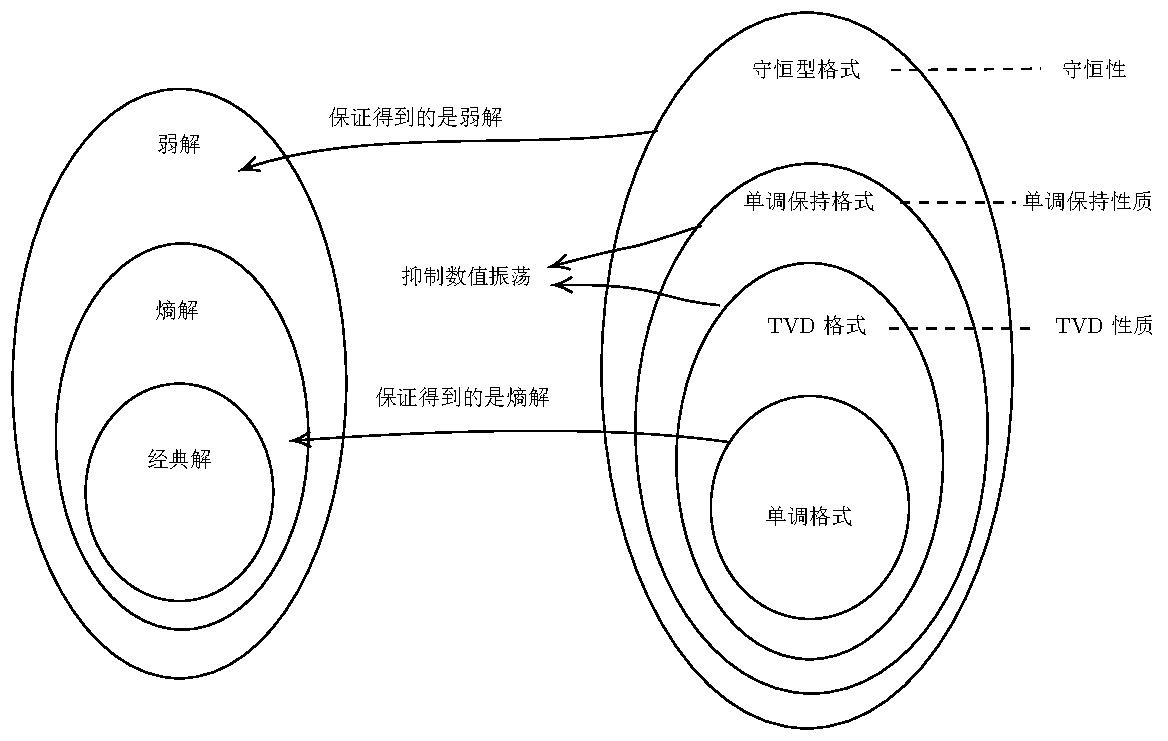
\includegraphics[width=\textwidth]{tikz/cv-schemes.pdf}
    \caption{守恒律方程的各种数值格式与各种解之间的关系} \label{fig:cv-schemes}
\end{figure}


\section{数值格式(二)}

前文中设计的数值格式具有如下特点:
\begin{enumerate}
    \item 基于流通分裂构造的 Lax-Friedrichs 格式是单调格式;
    \item 使用空间平均替换得到的 Lax 格式是单调格式;
    \item 基于 Roe 平均构造的 Roe 迎风格式是TVD格式,但不是单调格式;
    \item 基于时间泰勒展开得到的 Lax-Wendroff 格式是守恒型格式,但不是单调保持格式,可能产生数值振荡。
\end{enumerate}


\begin{example}\label{eg:lax-friedrichs}
    考虑基于流通分裂构造的 Lax-Friedrichs 格式,证明它是 TVD 格式。
\end{example}

\begin{proof}
    {\small
        \begin{align*}
            v_j^{n+1} ={} & v_j^n - \frac{\Delta t}{\Delta x}(f^+(v_{j}^n)-f^+(v_{j-1}^n))
            - \frac{\Delta t}{\Delta x}(f^-(v_{j+1}^n)-f^-(v_{j}^n))                       \\
            ={}           & v_j^n - \frac{\Delta t}{\Delta x}\left(
            f^+(v_{j}^n) + f^-(v_{j+1}^n) - f^+(v_{j-1}^n) - f^-(v_{j}^n)
            \right)                                                                        \\
            ={}           & v_j^n - \frac{\Delta t}{\Delta x}\left(
            \hat{f}_{j+\frac12}^n - \hat{f}_{j-\frac12}^n
            \right)
        \end{align*}}
    因此 Lax-Friedrichs 格式是守恒型格式,对应的数值流通量 $\hat{f}_{j+\frac12} = \hat{f}^{LF}(v_j^n,v_{j+1}^n)$ 称为 Lax-Friedrichs flux,具体定义为
    \[
        \hat{f}^{LF}(u^-,u^+) =
        f^+(u^-) + f^-(u^+) =
        \frac12(f(u^-)+f(u^+)) - \frac{\alpha}2 (u^+-u^-),\quad \alpha = \max |f'| \qedhere
    \]
\end{proof}


\begin{example}
    考虑基于流通分裂构造的 Lax-Friedrichs 格式,在满足 CFL 条件时,证明它是单调格式。
\end{example}

\begin{proof}
    \[
        v_j^{n+1} ={}  v_j^n - \frac{\Delta t}{\Delta x}(f^+(v_{j}^n)-f^+(v_{j-1}^n))
        - \frac{\Delta t}{\Delta x}(f^-(v_{j+1}^n)-f^-(v_{j}^n))   =:   H(v_{j-1}^n,v_j^n,v_{j+1}^n).
    \]
    单调性要求
    \begin{align*}
        \frac{\partial H}{\partial v^n_{j-1}} ={} & \frac{\Delta t}{2\Delta x}(f'(v^n_{j-1})+\alpha)\ge 0 , \\
        \frac{\partial H}{\partial v^n_{j}} ={}   & 1-\alpha\frac{\Delta t}{\Delta x}\ge 0,                 \\
        \frac{\partial H}{\partial v^n_{j+1}} ={} & \frac{\Delta t}{2\Delta x}(\alpha-f'(v^n_{j+1}))\ge  0
    \end{align*}
    $\alpha = \max |f'|$ 可以保证第一个和第三个不等式成立,第二个不等式即 CFL 条件。
\end{proof}

\begin{example}
    考虑使用空间平均替换得到的 Lax 格式,在满足 CFL 条件时,证明它是单调格式。
\end{example}

\begin{proof}
    \[
        v_j^{n+1} = \frac12 (v_{j-1}^n + v_{j+1}^n)
        - \frac{\Delta t}{2\Delta x} \left(f(v_{j+1}^n)-f(v_{j-1}^n)\right)  =:   H(v_{j-1}^n,v_j^n,v_{j+1}^n).
    \]
    单调性要求
    \[
        \frac{\partial H}{\partial v^n_{j-1}} ={}  \frac12(1 + \frac{\Delta t}{\Delta x}f'(v^n_{j-1}))
        \ge 0 ,\quad
        \frac{\partial H}{\partial v^n_{j}} ={}  0       ,\quad
        \frac{\partial H}{\partial v^n_{j+1}} ={} \frac12(1 - \frac{\Delta t}{\Delta x}f'(v^n_{j+1}))
        \ge 0
    \]
    CFL 条件 $\max |f'| \Delta t \le \Delta x$ 可以保证第一个和第三个不等式成立。
\end{proof}


\begin{example}
    对于 Engquist-Osher 格式
    \[
        v_j^{n+1} = v_j^n - \frac{\Delta t}{\Delta x}\left( \hat{f}_{j+\frac12}^n - \hat{f}_{j-\frac12}^n \right)
    \]
    其中的数值流通量 $\hat{f}_{j+\frac12}^n = \hat{f}^{EO}(v_j^n,v_{j+1}^n)$ 定义为
    \[
        \hat{f}^{EO}(u^-,u^+) = \frac{f(u^-) + f(u^+)}2 - \frac12 \int_{u^-}^{u^+} |f'(v)| dv
    \]
    在满足 CFL 条件时,证明它是单调格式。
\end{example}

\begin{proof}
    对数值流通量求导可得
    \begin{align*}
        \partial_1 \hat{f}^{EO}(u^-,u^+) & = \frac{f'(u^-) + |f'(u^-)|}2 \ge 0, \\
        \partial_2 \hat{f}^{EO}(u^-,u^+) & = \frac{f'(u^+) - |f'(u^+)|}2 \le 0.
    \end{align*}
    单调性要求
    \begin{align*}
        \frac{\partial H}{\partial v^n_{j-1}} ={} & \frac{\Delta t}{\Delta x} \partial_1 \hat{f}^{EO}(v_{j-1}^n,v^n_{j}) \ge 0   \\
        \frac{\partial H}{\partial v^n_{j}} ={}   & 1 - \frac{\Delta t}{\Delta x}
        \left[
            \partial_1 \hat{f}^{EO}(v_{j}^n,v^n_{j+1}) - \partial_2 \hat{f}^{EO}(v_{j-1}^n,v^n_{j})
        \right]  = 1 - \frac{\Delta t}{\Delta x} |f'(v_j^n)| \ge 0                                                               \\
        \frac{\partial H}{\partial v^n_{j+1}} ={} & - \frac{\Delta t}{\Delta x} \partial_2 \hat{f}^{EO}(v_{j}^n,v^n_{j+1}) \ge 0
    \end{align*}
    CFL 条件 $\max |f'| \Delta t \le \Delta x$ 可以保证第二个不等式成立。
\end{proof}

\begin{example}
    考虑基于 Roe 平均构造的 Roe 迎风格式,在满足 CFL 条件时,证明它是TVD格式。
\end{example}

\begin{proof}
    {\small
        \begin{align*}
            v_j^{n+1} ={} & v_j^n - \frac{\Delta t}{2\Delta x}
            (1+\text{sgn}(a_{j-\frac12}^n))(f(v_{j}^n)-f(v_{j-1}^n))
            - \frac{\Delta t}{2\Delta x} (1-\text{sgn}(a_{j+\frac12}^n))(f(v_{j+1}^n)-f(v_{j}^n))                                                            \\
            ={}           & v_j^n - \frac{\Delta t}{2\Delta x}
            (1+\text{sgn}(a_{j-\frac12}^n))\frac{f(v_{j}^n)-f(v_{j-1}^n)}{v_{j}^n-v_{j-1}^n}(v_{j}^n-v_{j-1}^n)                                              \\
                          & - \frac{\Delta t}{2\Delta x} (1-\text{sgn}(a_{j+\frac12}^n))\frac{f(v_{j+1}^n)-f(v_{j}^n)}{v_{j+1}^n-v_{j}^n}(v_{j+1}^n-v_{j}^n) \\
            =:{}          & v_j^n - C_{j-\frac12}(v_j^n - v_{j-1}^n) + D_{j+\frac12}(v_{j+1}^n - v_j^n)
        \end{align*}}
    其中
    \begin{align*}
        C_{j-\frac12} & = \frac{\Delta t}{2\Delta x}
        (1+\text{sgn}(a_{j-\frac12}^n))\frac{f(v_{j}^n)-f(v_{j-1}^n)}{v_{j}^n-v_{j-1}^n}
        = \frac{\Delta t}{2\Delta x}
        (1+\text{sgn}(a_{j-\frac12}^n)) a_{j-\frac12}^n \,\ge 0 , \\
        D_{j+\frac12} & = - \frac{\Delta t}{2\Delta x}
        (1-\text{sgn}(a_{j+\frac12}^n))\frac{f(v_{j+1}^n)-f(v_{j}^n)}{v_{j+1}^n-v_{j}^n}
        = -\frac{\Delta t}{2\Delta x}
        (1-\text{sgn}(a_{j+\frac12}^n)) a_{j+\frac12}^n \,\ge 0 ,
    \end{align*}
    并且
    \[
        C_{j+\frac12} + D_{j+\frac12}
        ={}  \frac{\Delta t}{2\Delta x} a_{j+\frac12}^n
        (1+\text{sgn}(a_{j+\frac12}^n)-1+\text{sgn}(a_{j+\frac12}^n))
        ={} \frac{\Delta t}{\Delta x}
        \text{sgn}(a_{j+\frac12}^n)  a_{j+\frac12}^n \le 1
    \]
    对应为 CFL 条件:$\text{max}|a_{j+\frac12}^n| \, \Delta t \le \Delta x$。
\end{proof}

\begin{remark}
    即使在满足 CFL 条件时,Roe 迎风格式也不是单调格式。
\end{remark}


\begin{example}
    Lax-Wendroff 格式是守恒型格式。
\end{example}

\begin{proof}
    \begin{align*}
        v_j^{n+1} ={} & v_j^n
        - \frac{\Delta t}{2\Delta x} \left(f(v_{j+1}^n)-f(v_{j-1}^n)\right)
        \\ & + \frac{\Delta t^2}{2\Delta x^2}\left\{
        A_{j+\frac12}^n [f(v_{j+1}^n) - f(v_{j}^n)]
        - A_{j-\frac12}^n [f(v_{j}^n) - f(v_{j-1}^n)]
        \right\}
        \\
        ={}           & v_j^n - \frac{\Delta t}{\Delta x}
        \Big\{
        \left(\frac12(f(v_j^n)+f(v_{j+1}^n)) - \frac{\Delta t}{2\Delta x} A_{j+\frac12}^n[f(v_{j+1}^n) - f(v_{j}^n)]\right)
        \\ & -
        \left(\frac12(f(v_{j-1}^n)+f(v_{j}^n)) - \frac{\Delta t}{2\Delta x} A_{j-\frac12}^n[f(v_{j}^n) - f(v_{j-1}^n)]\right)
        \Big\}                                                  \\
        =:{}          & v_j^n - \frac{\Delta t}{\Delta x}\left(
        \hat{f}_{j+\frac12}^n - \hat{f}_{j-\frac12}^n
        \right)
    \end{align*}
    因此 Lax-Wendroff 格式是守恒型格式,对应的数值流通量 $\hat{f}_{j+\frac12}$ 为
    \[
        \hat{f}_{j+\frac12} = \frac12(f(v_j^n)+f(v_{j+1}^n)) - \frac{\Delta t}{2\Delta x} A_{j+\frac12}^n[f(v_{j+1}^n) - f(v_{j}^n)] \qedhere
    \]
\end{proof}

\begin{remark}
    数值实验表明,Lax-Wendroff 格式可能产生数值振荡,因此它不是单调保持格式。
\end{remark}
